\documentclass[svgnames,tikz]{standalone}
\usetikzlibrary{patterns,calc}



\begin{document}

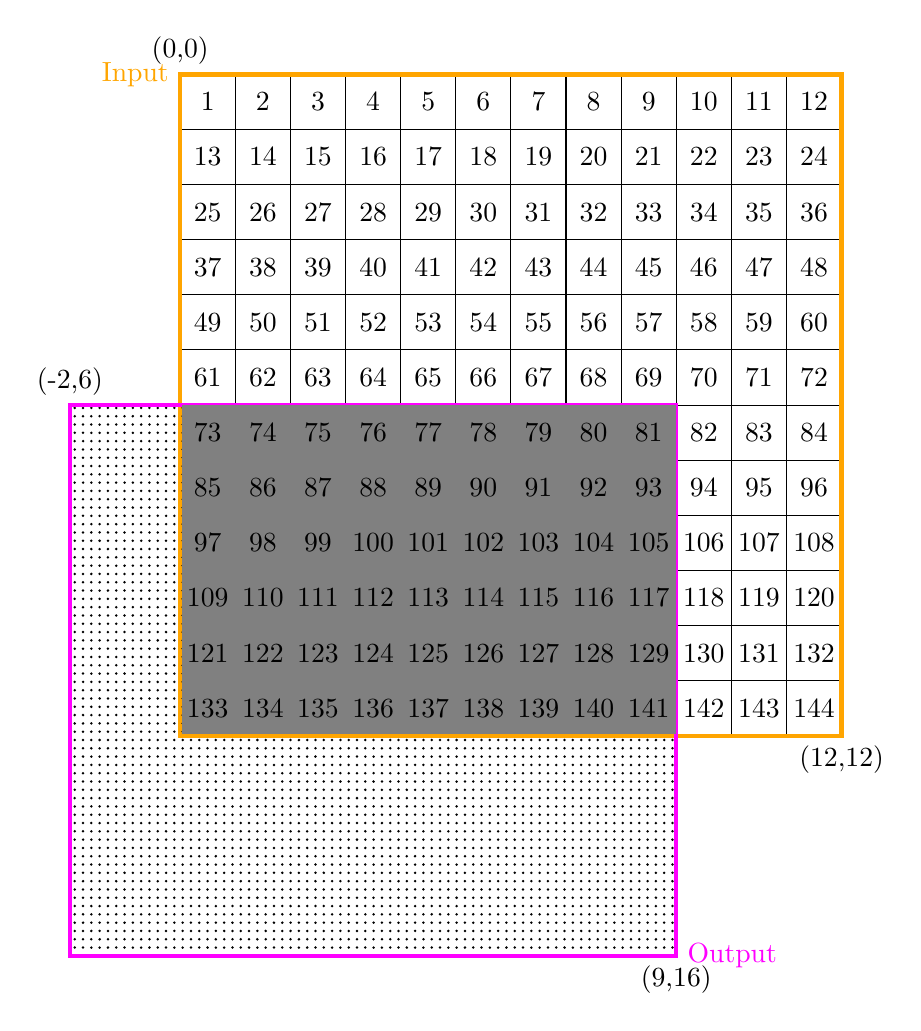
\begin{tikzpicture}[scale=.7,yscale=-1]
\tikzset{
  pad/.style={fill=LightGray},
  border/.style={very thick,<->}
}


\draw[fill=white] (0,0) grid[] (12,12);
\draw[ultra thick, Orange] (0,0) node[left] {Input} rectangle (12,12);
\draw[ultra thick, Magenta, pattern=dots] (-2,6) rectangle ++(11,10) node[right] {Output};

\node[above] at (0,0) {(0,0)};
\node[below] at (12,12) {(12,12)};
\node[above] at (-2,6) {(-2,6)};
\node[below] at (-2+11,6+10) {(9,16)};


\begin{scope}
  \clip (1pt,1pt) rectangle ($ (12,12) - (1pt,1pt) $);
  \fill[Gray] (-2,6) rectangle ++(11,10);
\end{scope}




\foreach \i in {0,...,11}{
\foreach \j in {1,...,12}{
  \draw let \n1 = {int(\i*12+\j)} in node at (\j-.5,\i+.5) {\n1};
}}



\end{tikzpicture}

\def\f#1#2{int((#2)*12+(#1)+1)}

\def\trunc#1{(#1) >= 0 ? (((#1) < 12) ? (#1) : 11) : 0}
\def\wrap#1{Mod(#1, 12)}
\def\mirrorB#1{(#1) >= 12 ? (23 - (#1)) : (#1)}
\def\mirror#1{\mirrorB{Mod(#1,24)}}
\def\padding#1#2#3{\f{#1{#2}}{#1{#3}}}
\def\inR#1{(#1 >= 0 && #1 < 12)}
\def\fillA#1#2{(\inR{#1} && \inR{#2}) ? \f{#1}{#2} : 69}



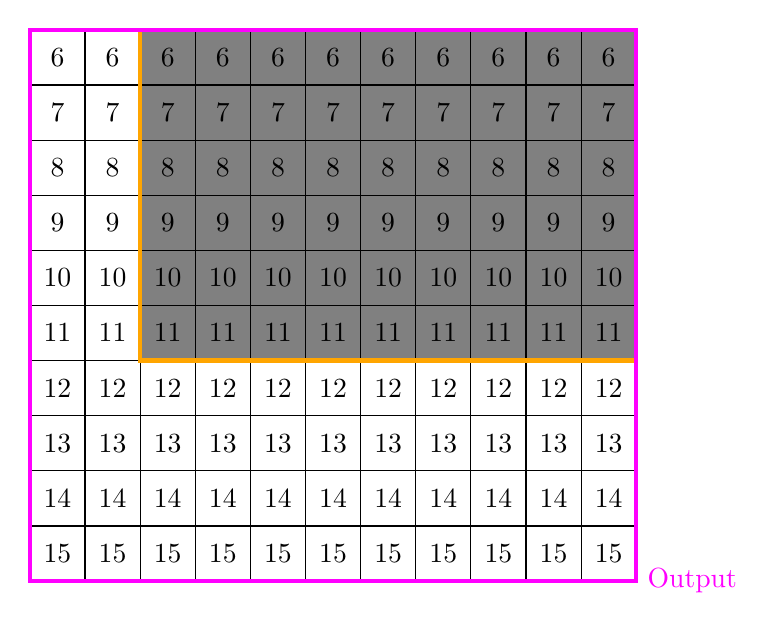
\begin{tikzpicture}[scale=.7,yscale=-1]
  \coordinate (A)  at (0,6);
  \coordinate (C)  at (9,12);

  
  \fill[Gray] (0,6) rectangle ++(9,6);
  \draw (-2,6) grid[] ++(11,10);
  \draw[Orange, ultra thick] (A) |- (C);
  \draw[ultra thick, Magenta] (-2,6) rectangle ++(11,10) node[right] {Output};


\foreach \yy in {6,...,15}{
  \foreach \xx in {-2,...,8}{
    \edef\mycmd{\padding{\wrap}{\xx}{\yy}}%
    %\show\mycmd%
    %
    \draw let \n1 = {\mycmd } in node at (\xx+.5,\yy+.5) {\n1};
}}
\end{tikzpicture}



\begin{tikzpicture}[scale=.7,yscale=-1]
  \fill[Gray] (0,6) rectangle ++(9,6);
  \draw (-2,6) grid[] ++(11,10);
  \draw[Orange, ultra thick] (A) |- (C);
  \draw[ultra thick, Magenta] (-2,6) rectangle ++(11,10) node[right] {Output};


\foreach \yy in {6,...,15}{
  \foreach \xx in {-2,...,8}{
    \edef\mycmd{\padding{\mirror}{\xx}{\yy}}%
    %\show\mycmd%
    %
    \draw let \n1 = {\mycmd } in node at (\xx+.5,\yy+.5) {\n1};
}}
\end{tikzpicture}

\begin{tikzpicture}[scale=.7,yscale=-1]
  \fill[Gray] (0,6) rectangle ++(9,6);
  \draw (-2,6) grid[] ++(11,10);
  \draw[Orange, ultra thick] (A) |- (C);
  \draw[ultra thick, Magenta] (-2,6) rectangle ++(11,10) node[right] {Output};

\foreach \yy in {6,...,15}{
  \foreach \xx in {-2,...,8}{
    \edef\mycmd{\padding{\trunc}{\xx}{\yy}}%
    %\show\mycmd%
    %
    \draw let \n1 = {\mycmd } in node at (\xx+.5,\yy+.5) {\n1};
}}
\end{tikzpicture}

\begin{tikzpicture}[scale=.7,yscale=-1]
  \fill[Gray] (0,6) rectangle ++(9,6);
  \draw (-2,6) grid[] ++(11,10);
  \draw[Orange, ultra thick] (A) |- (C);
  \draw[ultra thick, Magenta] (-2,6) rectangle ++(11,10) node[right] {Output};


\foreach \yy in {6,...,15}{
  \foreach \xx in {-2,...,8}{
    \edef\mycmd{\fillA{\xx}{\yy}}%
    %\show\mycmd%
    %
    \draw let \n1 = {\mycmd } in node at (\xx+.5,\yy+.5) {\n1};
}}
\end{tikzpicture}





\end{document}

